
\documentclass[a4paper, oneside, 11pt]{report}
\usepackage{epsfig,pifont,float,amsmath,amssymb, url, graphicx}
\newcommand{\mc}{\multicolumn{1}{c|}}
\newcommand{\mb}{\mathbf}
\newcommand{\mi}{\mathit}
\newcommand{\oa}{\overrightarrow}
\newcommand{\bs}{\boldsymbol}
\newcommand{\ra}{\rightarrow}
\newcommand{\la}{\leftarrow}
\topmargin = 0pt
\voffset = -80pt
\oddsidemargin = 15pt
\textwidth = 425pt
\textheight = 750pt
\usepackage[parfill]{parskip}

\begin{document}

\begin{titlepage}
\begin{center}
\rule{12cm}{1mm} \\
\vspace{1cm}
{\large  CMP-7009A Advanced Programming Concepts and Techniques}
\vspace{7.5cm}
\\{\Large Project Report - 14 November 2018}
\vspace{1.5cm}
\\{\LARGE Evolution Sandbox}
\vspace{1.0cm}
\\{\Large Group members: \\ Benjamin Longhurst, Rupert Hammond, Ryan Phelan, Travis Payne}
\vspace{10.0cm}
\\{\large School of Computing Sciences, University of East Anglia}
\\ \rule{12cm}{0.5mm}
\\ \hspace{8.5cm} {\large Version 1.0}
\end{center}
\end{titlepage}

\setcounter{page}{1}
%\pagenumbering{roman}
%\newpage

\begin{abstract}
	
\end{abstract}

\chapter{Introduction}
The Evolution Simulation attempts to represent the way a set of organisms evolve within a limited ecosystem. This is achieved by utilising a variety of programming concepts and techniques such as Multi-threading, Dijkstra's A* algorithm, genetic crossover algorithm, finite state machines and tile based movement. These techniques hope to demonstrate chosen aspects of evolution within a sandbox environment.

\section{Aims and Objective}
The aim of this project is to produce a graphical evolutionary simulation with some degree of interactivity. In order to meet this objective, a set of requirements were produced:
\begin{itemize}\label{requirements}
	\item Organisms should act based on personal attributes, similar to the rule system in Conway's Game of Life
	\item Organism attributes should be customisable on the fly
	\item Organism attributes should mutate over generations using a crossover algorithm
	\item Organisms should utilize logical path finding when seeking out their objectives
	\item The ecosystem should reach equilibrium when left to its own devices
	\item The simulation should be able to handle a large number of organisms without noticeable lag
	\item The simulation should employ realistic biological algorithms where possible
	\item The UI should be clean, simple and professional
	\item The graphics should faithfully represent the underlying simulation
\end{itemize}

\section{MoSCoW}
To better understand the scope and priorities of the project, a MoSCoW analysis was produced (Figure~\ref{moscow}). In general, the ``Must Have`` objectives are those identified to be necessary for an end-to-end functioning product, while ``Should Have`` is considered a bare minimum submission. ``Could Have`` contains a mix of objectives such as spritesheet animation would improve the simulation quality but are not necessarily crucial, or otherwise those such as speciation which would substantially increase the simulation complexity. The implementation of this analysis is discussed in detail within Section~\ref{versioning}.
\smallskip 

\begin{figure}[H]
	\caption{MoSCoW Analysis}\label{moscow}
	\centering
	\begin{tabular}{c|p{0.8\textwidth}}
		Must Have & \begin{itemize}
			\itemsep0em
			\item Organism life cycle
			\item Genetic crossover algorithm
			\item Unique organism attributes such as health, age, strength, speed and resistances
			\item Organisms state determined by their unique attributes
			\item Unique organism attributes should be editable on the fly
			\item Simple UI Overlay
			\item Live edit of organisms
			\item Simple 2D graphics
			\item Herbivores and natural food sources
		\end{itemize} \\ \hline
		Should Have & \begin{itemize}
			\itemsep0em
			\item Weather/disease system
			\item Advanced path-finding algorithm
			\item Carnivores and predator/prey organisms
			\item Terrain variation, e.g. grass, mountainous, water
			\item Ability to pause, speed up and slow down simulation
		\end{itemize} \\ \hline
		Could Have & \begin{itemize}
			\itemsep0em
			\item Natural disasters
			\item Speciation (new species forming from heavily mutated organisms over time)
			\item A game log with charts and text output
			\item Spritesheet animation
			\item Particle effects, e.g. weather effects, running water, blood
			\item Program flow (start screen, simulation setup, end screen etc.)
		\end{itemize} \\ \hline
		Won't Have & \begin{itemize}
			\itemsep0em
			\item 3D graphics
			\item Scale realism
		\end{itemize} \\
	\end{tabular}
\end{figure}

\section{Report structure}
This report will cover a brief background of evolution and the algorithms which attempt to simulate it in Section~\ref{background}. Section~\ref{methodology} details the various advanced programming and project management techniques utilized in the project. Models and implementation details are outlined in Section~\ref{implementation}. Finally, the product's quality will be tested and verified through experiments in Section~\ref{testing} before being drawn to a conclusion in Sections \ref{discussion} and \ref{conclusion}.

\chapter{Background}\label{background}
[TODO: I'm not sure Conway's Game of Life should be the focus anymore]

One such example of an evolution simulation is Conway's Game of Life. Created in 1970 by John Conway, the simulation takes place on an infinitely sized grid where each cell is either live or dead. It progresses according to a set of simple rules \cite{guardian}:
\begin{itemize}
	\item A live cell with less than two live neighbours becomes dead
	\item A live cell with more than four live neighbours becomes dead
	\item A dead cell with three live neighbours become alive
\end{itemize}

Conway's Game of Life is often praised for its ability to show how simple rules can spawn complex evolutionary patterns \cite{callahan}. This project will tackle evolution simulating by taking inspiration from Conway's Game of Life to produce a piece of software it terms an ``evolution sandbox``; a simulation with emphasis on real-time manipulation and customization which will allow the user to observe the outcome of their actions on the ecosystem.

\chapter{Methodology}\label{methodology}

\section{Agile Methodology}\label{projectmanagement}
The project is managed according to Agile principles by implementing the Scrum framework. At most points in the project, meetings occurred twice per week (one lab session, one outside) and would begin with a short stand-up meeting. Iterative version releases were promoted with the rule that all feature branches should be merged into master before the week's lab meeting. Development as a whole was split into several versions (Section~\ref{versioning}), which were tackled in two to three week sprints. GitHub was used as the centre for project management through a combination of it's Git Project Boards feature, where each board corresponds to one sprint and therefore one product version (Figure~\ref{gitboard}), and it's issue tracking (Figure~\ref{gitissue}). 

\begin{figure}[H]
	\caption{GitHub Project Board}\label{gitboard}
	\centering
	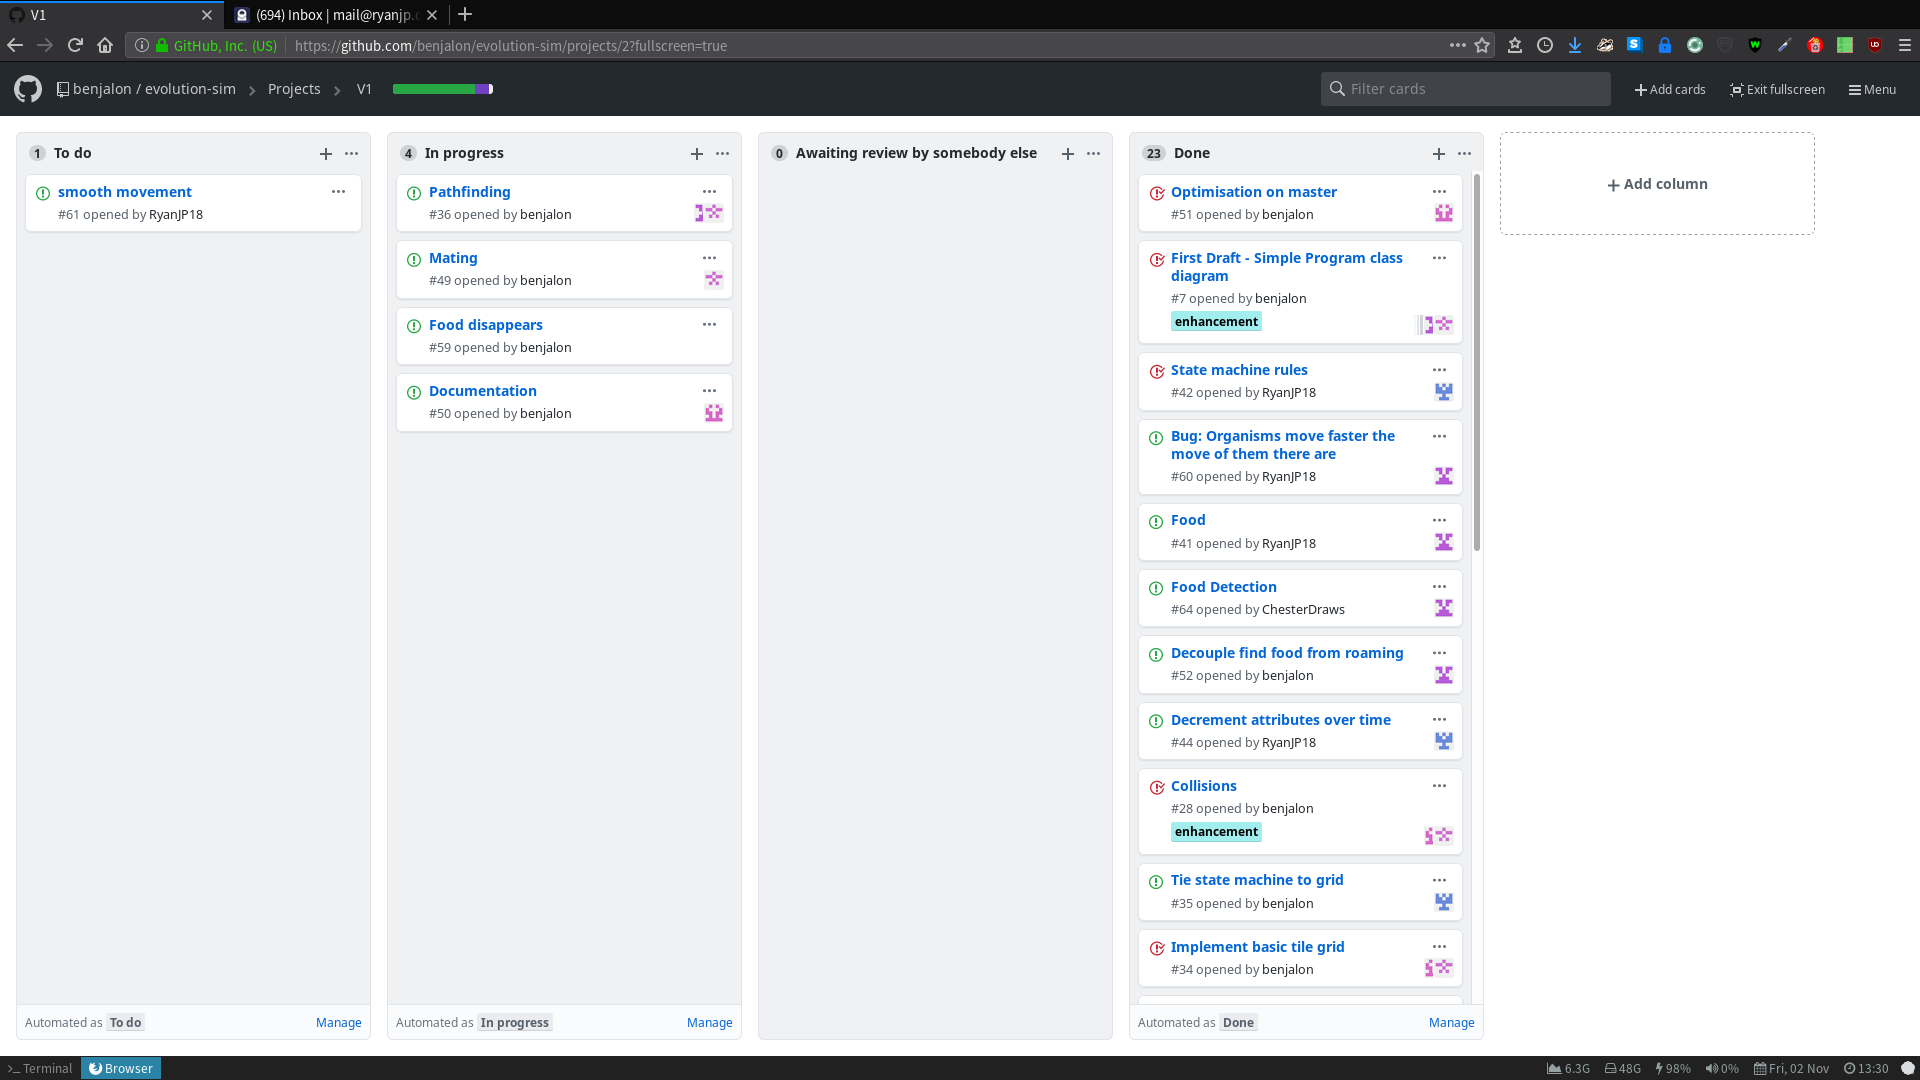
\includegraphics[width=1\textwidth]{gitproj}
\end{figure}

\begin{figure}[H]
	\caption{GitHub Issue Tracking}\label{gitissue}
	\centering
	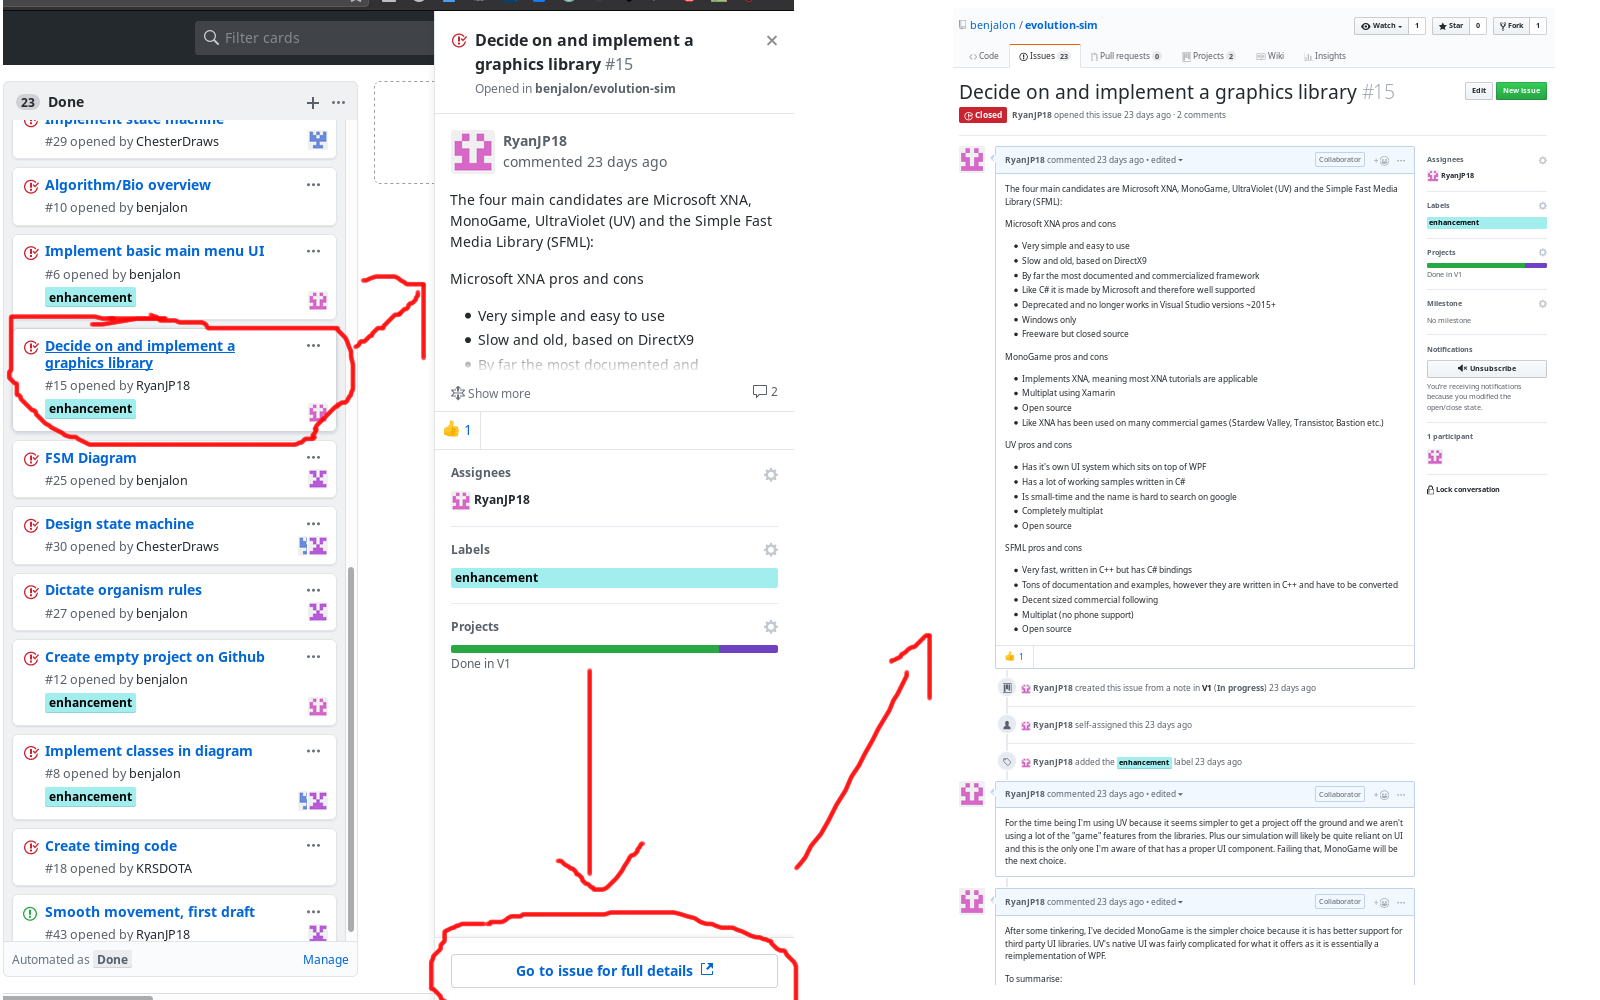
\includegraphics[width=1\textwidth]{gitissuetrack}
\end{figure}

Using Git, each ticket is developed on a unique feature branch. When code-complete, it is sent for pull request (i.e. peer review) before it can be merged into master. This system is enforced through a merge lock on master which only allows branch merges as opposed to direct commits. Additionally, these merges are rejected by the system unless it is reviewed by one other person. This system helps ensure the quality of master for branching at all times, avoiding situations where development is halted due to a buggy code-base. Additionally, these pull requests are able to function as a form of white-box testing as discussed in (Section~\ref{testing}).

Other project management tools used throughout the project include Microsoft OneNote for collaborative documentation and WhatsApp for quick discussion and meeting scheduling.

\section{Code Architecture}\label{architecture}
The SOLID principles define five guidelines which are used as the guiding principles in the project's architecture to ensure that code is maintainable and easy to understand \cite{kelmendi}:
\begin{itemize}
	\item Single Responsibility: Every class should have only one responsibility to prevent the class being susceptible to requirement changes.
	\item Open-Closed: Classes should be open to extension but abstraction should be used to avoid the need for rewrites on the extended code.
	\item Liskov Substitution: Derived and base classes should be substitutable.
	\item Interface Segregation: Keep interfaces simple to avoid bulk from implementing unnecessary properties.
	\item Dependency Inversion: Keep abstract code abstract by avoiding dependencies on low level code.
\end{itemize}

An example of how this has influenced design can be seen in the choice to split Grid from StateMachine within their use inside Simulation. Although both handle moving and positioning organisms, Grid is treated as the ``graphical brain``, positioning organisms and drawing them at their positions, whereas the StateMachine is used as the ``logical brain``, dictating the behaviour which causes the organisms to be repositioned in the first place. This separation of concerns can also be seen in the namespaces, for example EvolutionSim.StateMachine, EvolutionSim.TileGrid, EvolutionSim.Data and EvolutionSim.UI.

Another example is through having GridItem function as a base class for Organism and Food. This swappable base is important due to the Tiles of Grid accepting either as a potential inhabitant. This swappable nature would not work if the Liskov Substitution principle was not applied.

To ensure a clean and consistent code-base, the official Microsoft C\# conventions are applied where possible. Notable examples include placing braces on a new line, using camelCase for variable names and avoiding one line if statements \cite{microsoft}.

\section{State Management}\label{statemanagement}
Within the simulation all organism behaviour is dictated by a finite state machine which contains a set of states and rules for moving between them. The StateMachine class is passed State objects which are essentially a lookup table for each state transition. Transitions use a pair of enum values, OrganismState and Action, where OrganismState refers to the current state of the Organism and Action is the event responsible for causing the transition. Based on this supplied information, the StateMachine determines which state the Organism should transition to and throws an exception if it determines the move to be illegal, for example it is impossible for an Organism to move directly from ``Mating`` to ``Eating`` through the Action ``FoundFood`` as the Organism must be in the ``Roaming`` state in order to reach this clause.

In addition to these state management tasks, the StateMachine also contains two methods to drive organism behaviour: CheckState and DetermineBehaviour, which are both called every cycle of the Update loop. CheckState is responsible for checking that each Organism is in the correct state based on the rules defined for the simulation, for example if an organism is currently in the ``Roaming`` state, but it's hunger levels have dropped below 0.4, this would mean that the organism must now move into ``SeekingFood``. After the state is checked, DetermineBehaviour defines how the Organism should behave within this state.

\section{Crossover Algorithm}\label{crossover}
TODO

\section{Tile-Based Movement}\label{grid}
A common method of implementing movement in a simulation is by constraining it to a grid. This is useful because the number of movement states becomes finite and better lends itself to algorithms for path-finding. In terms of efficiency, a grid also reduces the need for collision detection between simulation elements by mediating on the movement between tiles. Linear interpolation is also applied to all tiles movements so that the organisms move smoothly rather than ``teleporting`` between them.

Within code, the Grid class holds a collection of Tiles within a jagged array which can each potentially hold a GridItem inhabitant. Within this collection, each index maps the tile to a screen position using the equation:
\[tilePos = offset + (tileIndex * TILE_SIZE)\]

\section{Pathfinding Algorithm}\label{pathfinding}
Pathfinding is a key component in the simulation and three main methods were considered for it: depth first search (DFS), Dijkstra's algorithm and the A* algorithm. In terms of simplicity, DFS produces fast results but is naive and requires a large amount of time and memory to find the shortest route. Dijkstra's algorithm is an improvement because it applies a difficulty based on the movement cost to a destination, but is expensive as it compares equally and needlessly expands difficult locations without considering direction. Finally, at least for single-point to single-point searches (as used in this project), A* is considered the fastest algorithm \cite{belwariar} due to its improvement upon Dijkstra's with a heuristic. 
\[A* Algorithm: f(n) = g(n) + h(n)\]
In the above formula g(n) refers to the difficulty of a tile which is an important consideration in handling different terrain types such as hills or water. The h(n) is the diagonal distance between the two points and f(n) refers to the sum of g(n) and h(n).

A* is implemented in code by creating a Node object for each Tile, each holding a reference to the previous Node, its Grid position, the destination's distance and the difficulty in reaching it. To calculate the g(n) difficulty value, the terrain type of the Tile is taken into account and for the h(n) distance value, the diagonal distance between the two points is calculated by taking the maximum value of either the goal Tile's x coordinate minus the current Tile's x coordinate or the same for y coordinates. Nodes to be evaluated are stored in open and closed collections which are manipulated until a path to the goal is found.

\section{Optimisation}\label{optim}
Optimisation is important for the project due to its requirement in handling a large number of organisms without noticeable lag. By default, MonoGame's render loop updates and draws at sixty frames per second. Should the update logic fail to complete within this ~16-17ms time-frame then it delays the draw call, which lowers the simulation's frame-rate. This has further knock-on effects where the draw calls become progressively more delayed and eventually cause input lag on the UI. As the update method is essentially the primary path through the code, it calls into several loops to cycle through the items which make up the simulation. There can be several hundred objects to iterate through during any given Update loop and keeping this entire iteration within the acceptable ~16-17ms limit required a great deal of optimisation. Despite this, optimisation was a task left until it became a problem following the argument that ``premature optimization is the root of all evil [...]`` \cite{knuth} by introducing bugs and making code less readable. 

As the simulation grew in size, loop optimisation became an issue particularly for state management and path finding. To improve this, variables are typically declared outside of loop scope to prevent them being redeclared on each iteration. Other standard optimisations such as caching the collection length ahead of time and avoiding high precision calculations are also applied. The grid's collection for storing tile objects is also a jagged array as opposed to a multi-directional one which is more efficient to loop over.

From an more architectural perspective, the grid system is also a form of optimisation. By constricting organism movements to a grid the simulation is able to cut down on the need for collision detection, which would otherwise have been a bottleneck for the system. This would have required exponentially more computation as organisms are added because each organism would need to check the itself against all others.

\section{Multi-threading}
TODO.

\chapter{Implementation} \label{implementation}

\subsection{Modelling}

TODO OOA and UML

The class diagram Figure~\ref{classdiagram} was continually updated throughout the project and although it saw many changes, certain key themes remained constant throughout.

An architectural decision was to ensure the separation of concerns between the graphics, states, simulation and UI. The graphical component provides a representation of the simulation's output, but they are kept unaware of the inner workings of the other to better decouple their behaviour. Likewise, while the UI can interact with the simulation, there was no need to have this behaviour tied in any way to the intricacies of it. As such, the relationship between the three key areas can be observed as limited on the class diagram.

Another theme present in the class diagram is abstraction. Through inheritance, GridItems are kept as generic inhabitants by the Tiles of the Grid. This means that the Grid can manage its Tiles and their inhabitant GridItems without particular knowledge of whether they are Organisms or Food or Obstacles, simplifying the implementation.

\section{Tools}\label{tools}
Three programming languages were considered for the project: C++, C\# and Java. The simulation was identified to have a large dependency on computation due to the fact that there could be upwards of one hundred organisms on screen at any one time and each of them would require state management, path finding and collision detection. For this reason, C++ seemed to be the natural choice due to the speed benefit of dynamic memory management. However, upon further research it was found that C\# had a more diverse set of 2D graphics libraries with C++ libraries typically focused on 3D rendering. Finally, Java was considered because the bulk of the team's experience was with the language, though because C\# can be used as a drop-in replacement for Java this was seen as another benefit in using C\#.

A comparison was made between several popular 2D graphics libraries available in C\#, shown in Figure~\ref{library-comparison}.

\begin{figure}[H]
	\caption{Graphics Library Comparison}\label{library-comparison}
	\centering
	\begin{center}
		\begin{tabular}{c|p{0.4\textwidth}|p{0.4\textwidth}}
			Library & Pros & Cons \\ \hline
			Microsoft XNA & \begin{itemize}
				\itemsep0em
				\item Simple and easy to use
				\item Very well documented
				\item Well-used commercially
				\item Supported by Microsoft who also made C\#
			\end{itemize} & \begin{itemize}
				\itemsep0em
				\item Slow and old, based on DirectX9
				\item Deprecated and no longer works in Visual Studio 2015+
				\item Windows only
				\item Closed source
			\end{itemize} \\ \hline
			MonoGame & \begin{itemize}
				\itemsep0em
				\item Based on XNA with the same syntax, all of the XNA documentation is applicable
				\item Multi-platform but requires Xamarin
				\item Open source
				\item Has seen use on commercial games (Stardew Valley, Transistor, Bastion etc.)
			\end{itemize} & \begin{itemize}
				\itemsep0em
				\item Convoluted asset management system
			\end{itemize} \\ \hline
			UV & \begin{itemize}
				\itemsep0em
				\item Has a built in UI framework based on Windows Presentation Foundation (WPF)
				\item Truly multi-platform
				\item Open source
			\end{itemize} & \begin{itemize}
				\itemsep0em
				\item Convoluted asset management system
				\item Limited documentation, small time
				\item Little to no commercial use
			\end{itemize} \\ \hline
			SFML & \begin{itemize}
				\itemsep0em
				\item Very fast, written in C++ but has C\# bindings
				\item Well documented
				\item Some commercial use
				\item Multi-platform but no phone support
				\item Open source
			\end{itemize} & \begin{itemize}
				\itemsep0em
				\item C\# bindings are slightly behind on updates
				\item Examples and documentation are written in C++ and require converting
				\item Syntax is not as simple as other frameworks
			\end{itemize} \\
		\end{tabular}
	\end{center}
\end{figure}

Though UV was initially chosen due to its built-in UI support, the lack of documentation and convoluted XML system for managing assets meant that MonoGame was used instead. The third party UI library GeonBit.UI was chosen because one of the project requirements [\ref{requirements}] was that the UI have a professional look and it also provided out of box support for radio buttons and lists.

\subsection{Product Versions}\label{versioning}
In keeping with the spirit of iterative development, the projects aim to produce a new product at the end of each sprint. This ensures that at any given time, the active project board matches the current release version. Each version aimed to iterate upon the previous release with features taken from further down the MoSCoW analysis (Figure~\ref{version-table}).

\smallskip 
\begin{figure}[H]
	\centering
	\begin{tabular}{c|p{0.7\textwidth}|l} \label{version-table}
		Version & Goal & Deadline \\ \hline
		0 & A proof of concept to test the chosen technologies & Tuesday week 2 \\ \hline
		1 & A fully functioning basic simulation with all of the ``Must Have`` components from the MoSCoW analysis & Friday week 6 \\ \hline
		2 & Improvements on V1 simulation and ``should have`` objectives: A* path-finding, improved crossover algorithm, carnivores and a better time system. & Friday week 8 \\ \hline
		3 & Path finding performance enhancements and bug fixes & Friday week 10 \\ \hline
		3 & More ``Should Have`` objectives and missing functionality. Primarily eating, dying, mating, terrain and a time system. & Friday week 12 \\ \hline
		4 & Final missing features: Weather system, carnivores and prey, particle effects. & Christmas \\ \hline
		5 & Loose ends, bug fixes and report updates. & Project deadline \\ \hline
	\end{tabular}
\end{figure}
\smallskip 

\section{Proof of Concept}
A proof of concept was made with the chosen technologies to avoid a situation where the UML modelling and code architecture was planned according to a language or tool which was a poor fit for the project. It aimed to simply draw a number of organisms to the screen using the chosen graphics framework which could be manipulated using a simple place-holder UI.

\begin{figure}[H]
	\caption{Proof of Concept}\label{poc}
	\centering
	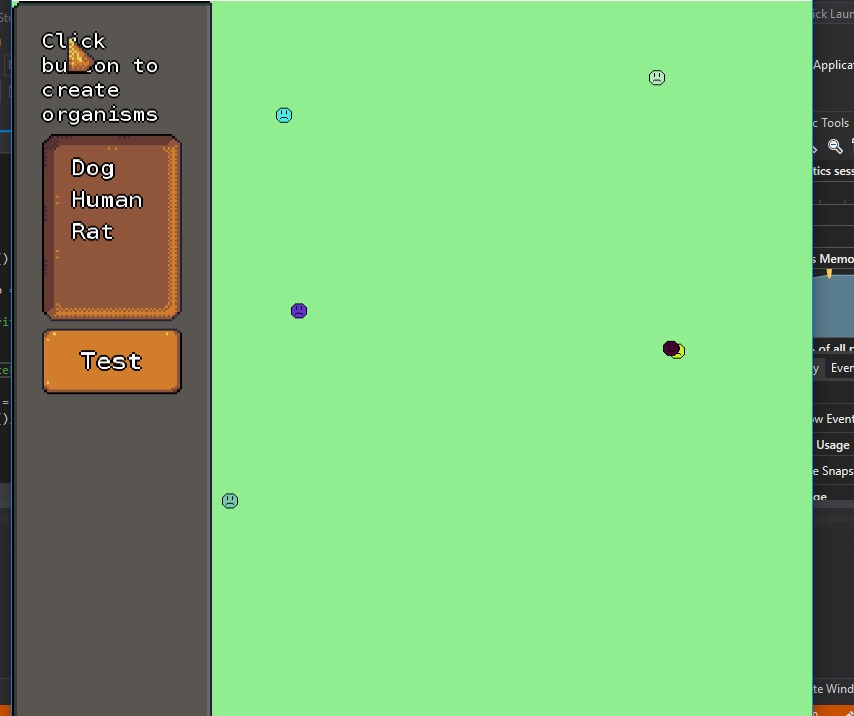
\includegraphics[width=0.8\textwidth]{poc}
\end{figure}

\chapter{Testing}\label{testing}

This section will be about the following:
\begin{itemize}
	\itemsep0em
	\item Pull requests as a form of white-box testing during development
	\item Unit testing with the built in C\# tools
	\item Experimenting with several untouched simulations to ensure equilibrium is reached 
	\item Experimenting with editing attributes and reaching equilibrium, likewise with natural disasters and disease
	\item A section on the bug fixing ticket system in place \label{bugfixing}
\end{itemize} 

\chapter{Discussion}\label{discussion}

This section will be about the following:
\begin{itemize}
	\itemsep0em
	\item Discussion of testing and experiment results
	\item Issues encountered: frequent rewrites, tangled state management early on, slowdown and lag, inconsistent coding standards, pathfinding necessitating optimisation and multiple threads, pull request system 
	\item What went well/badly
	\item What could be improved
\end{itemize} 

\chapter{Conclusion and Future Work}\label{conclusion}

This section will conclude the MoSCoW analysis, discuss shortcomings and future developments with more time. It will avoid subjective opinions, rants and excuses.

\bibliographystyle{unsrt}
\bibliography{references}

\chapter*{Contributions}

The team has agreed on a 25\% contibution each as of the time of writing. Note that these contributions are to date and not representative of planned features. 
\smallskip 
\begin{center}
	\begin{tabular}{c|p{0.4\textwidth}|p{0.4\textwidth}}
		Member & Ownership of/Major Contributions & Assisted on/Minor Contributions \\ \hline
		Benjamin Longhurst & \begin{itemize}
			\itemsep0em
			\item Project management [\ref{projectmanagement}]
			\item A* Pathfinding [\ref{pathfinding}]
		\end{itemize} & \begin{itemize}
			\itemsep0em
			\item Grid/tile system [\ref{grid}]
			\item Bio. algorithms research [\ref{crossover}]
		\end{itemize} \\ \hline
		Rupert Hammond & \begin{itemize}
			\itemsep0em
			\item State management [\ref{statemanagement}]
			\item State machine rules
			\item Bio. algorithms research [\ref{crossover}]
			\item Organism attributes
		\end{itemize} & \begin{itemize}
			\itemsep0em
			\item Bug fixing [\ref{bugfixing}]
			\item A* Pathfinding [\ref{pathfinding}]
		\end{itemize} \\ \hline
		Ryan Phelan & \begin{itemize}
			\itemsep0em
			\item Graphics/UI research and implementation [\ref{tools}]
			\item Grid/tile system [\ref{grid}]
			\item Optimisation [\ref{optim}]
			\item Report writing
		\end{itemize} & \begin{itemize}
			\itemsep0em
			\item Project management [\ref{projectmanagement}]
			\item Code architecture [\ref{architecture}]
		\end{itemize} \\ \hline
		Travis Payne & \begin{itemize}
			\itemsep0em
			\item Food system
			\item Movement logic
			\item Simulation flow [\ref{statemanagement}]
		\end{itemize} & \begin{itemize}
			\itemsep0em
			\item Code architecture [\ref{architecture}]
			\item Bug fixing [\ref{bugfixing}]
			\item A* Pathfinding [\ref{pathfinding}]
			\item Organism attributes
		\end{itemize} \\
	\end{tabular}
\end{center}
\smallskip
Other work such as the Proof of Concept, UML and analysis' were completed as a team with all members present.
\chapter*{Appendix A}

\begin{figure}[H]
	\caption{UML Class Diagram}\label{classdiagram}
	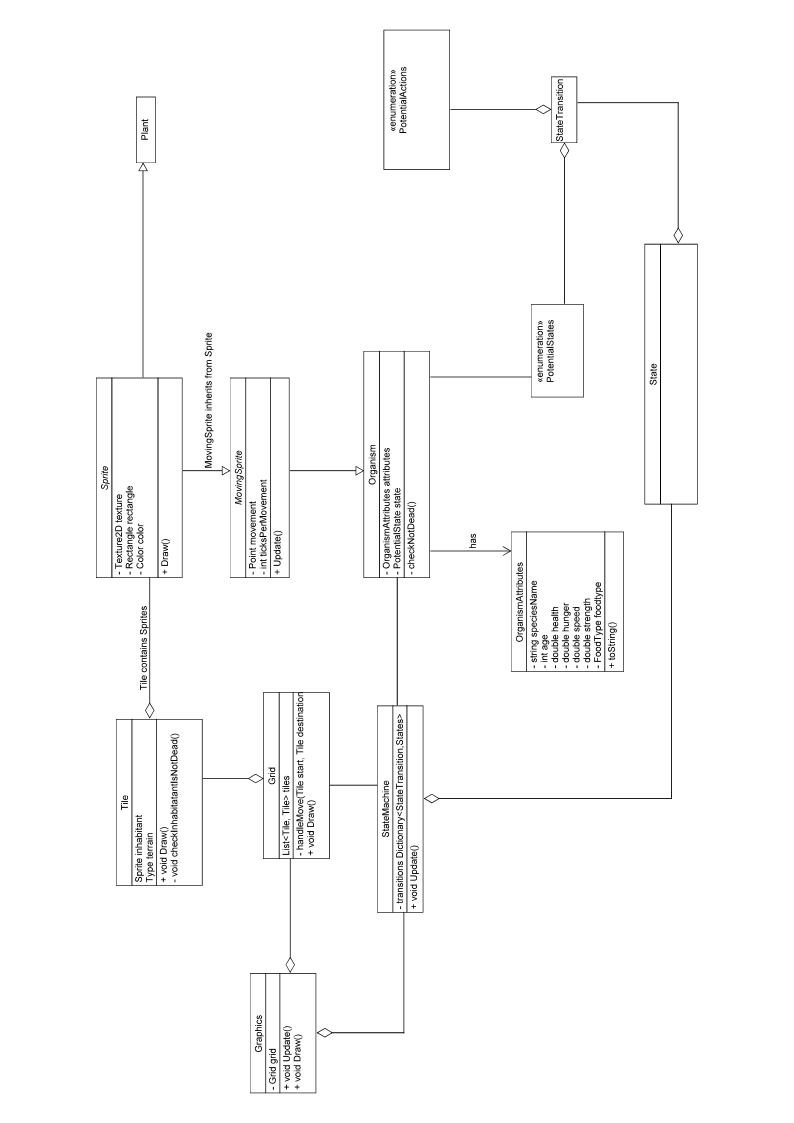
\includegraphics[width=\textwidth,height=\textheight]{class-diagram}
\end{figure}

\end{document}

